%%%%%%%%%%%%%%%%%%%%%%%%%%%%%%%%%%%%%%%%%%%%%%%%%%%%%%%%%%%%%%%%%%%%%%%%%%%%
% Sphere - A Multiplataform IDE for C++                                    %
% Copyright (C) 2006  Thiago dos Santos Alves                              %
%                                                                          %
% This program is free software; you can redistribute it and/or            %
% modify it under the terms of the GNU Lesser General Public               %
% License as published by the Free Software Foundation; either             %
% version 2.1 of the License, or (at your option) any later version.       %
%                                                                          %
% This program is distributed in the hope that it will be useful,          %
% but WITHOUT ANY WARRANTY; without even the implied warranty of           %
% MERCHANTABILITY or FITNESS FOR A PARTICULAR PURPOSE.  See the GNU        %
% Lesser General Public License for more details.                          %
%                                                                          %
% You should have received a copy of the GNU Lesser General Public         %
% License along with this library; if not, write to the Free Software      %
% Foundation, Inc., 51 Franklin St, Fifth Floor, Boston, MA 02110-1301 USA %
%                                                                          %
% Thiago dos Santos Alves disclaims all copyright interest in              %
% the program `Sphere' (a Multiplataform IDE for C++) written              %
% by him self.                                                             %
%                                                                          %
% Thiago dos Santos Alves, 22 February 2006                                %
% thiago.salves@gmail.com                                                  %
%%%%%%%%%%%%%%%%%%%%%%%%%%%%%%%%%%%%%%%%%%%%%%%%%%%%%%%%%%%%%%%%%%%%%%%%%%%%

\documentclass[11pt,a4paper]{report}
\usepackage[latin1]{inputenc}
\usepackage{amsmath}
\usepackage{amsfonts}
\usepackage{amssymb}
\usepackage[all]{xy}
\usepackage{paralist}

\usepackage{graphicx}

\author{Thiago dos Santos Alves}
\title{Technical Specification}
\begin{document}
\maketitle
\tableofcontents
\listoffigures

\begin{abstract}
This document will describe how the DevQt Editor solution will be implemented, what patterns, algorithms and whatever was necessary to do the dirty work should be used.
\end{abstract}

\chapter*{Preface}
\addcontentsline{toc}{chapter}{Preface}
bla bla bla bla bla bla bla bla bla bla bla bla bla bla bla 
bla bla bla bla bla bla bla bla bla bla bla bla bla bla bla 
bla bla bla bla bla bla bla bla bla bla bla bla bla bla bla 
bla bla bla bla bla bla bla bla bla bla bla bla bla bla bla 
bla bla bla bla bla bla bla bla bla bla bla bla bla bla bla 
bla bla bla bla bla bla bla bla bla bla bla bla bla bla bla 
bla bla bla bla bla bla bla bla bla bla bla bla bla bla bla 
bla bla bla bla bla bla bla bla bla bla bla bla bla bla bla 
bla bla bla bla bla bla bla bla bla bla bla bla bla bla bla 
bla bla bla bla bla bla bla bla bla bla bla bla bla bla bla 

\chapter{General Analisys} \label{generalAnalisys}
Looking into \cite{functional} I identify that the Editor's Widget should be divided into 5 parts that are classes that extends some \texttt{QWidget}:

\begin{enumerate}
\item Editor
\item LineNumberPanel
\item FoldPanel
\item LineMarksPanel
\item OverviewLineMarksPanel
\end{enumerate}

Of this parts, Editor is the main one. Each other part can access it and perform any desired action.

\section{Editor} \label{overviewEditor}
As the main part, this class should extend \texttt{QTextEdit} class and change the behaviour of it.

First we see that editor could work in four diferent states:

\begin{enumerate}
\item Normal
\item Persistent Selection
\item Multiline Edit
\item Persistent Selection with Multiline Edit
\end{enumerate}

The normal state is the behaviour of a normal \texttt{QTextEdit}\cite{qtDoc}, while Persistent Selection state and Multiline Edit state has its own behaviour that is described on \cite{functional}.

The Persistent Selection with Multiline Edit state, as you can imagine, is a state where user will has a persistent selection while he multiline editi his code.

Note that from state 1 it is possible to go to states 2 and 3 but never to the state 4, while in the state 4 it is only possible to go to states 2 and 3 too.

Figure~\ref{editorStates} will illustrate this:

\begin{figure}[hbt]
\begin{displaymath}
\xymatrix{
   & *++[F-:<13pt>]\txt{Normal \\ State} 
         \ar@/_1pc/[ld] \ar@/_1pc/[rd] \\
   *++[F-:<13pt>]\txt{Persistent \\ Selection \\ State} 
         \ar@/_1pc/[ru] \ar@/_1pc/[rd] &&
   *++[F-:<13pt>]\txt{Multiline \\ Edit \\ State} 
         \ar@/_1pc/[lu] \ar@/_1pc/[ld] \\
   & *++[F-:<13pt>]\txt{Multiline Edit \\with\\ Persistent Selection \\ State} 
         \ar@/_1pc/[lu] \ar@/_1pc/[ru]
}
\end{displaymath}
\caption{Possible states of editor} \label{editorStates}
\end{figure}

As its possible to represent editor with a stateful graph it is a great idea to use the State Pattern \cite{designPatterns} to implement it. With this, each state of the editor do its work on a independent way. Figure~\ref{statePattern} will illustrate this:

\begin{figure}[hbt]
\centering
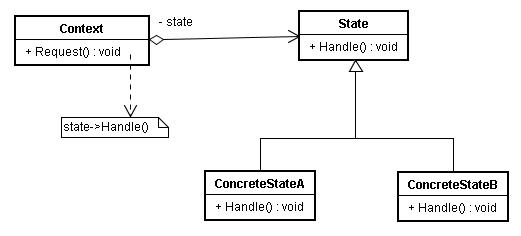
\includegraphics{images/state_pattern.jpg}
\caption{State Pattern Diagram} \label{statePattern}
\end{figure}

\section{LineNumberPanel} \label{linenumberOverview}
This \textit{widget} shows lines number relative to visible lines on the editor. Folded lines shuld be counted as lines too, so, this class should \textit{ask} to the ``Matcher'' extention if a line is collapsed, and if is the next line number must be the actual line number plus number of collapsed lines:
\begin{displaymath}
nextLine = lineNumber + LINES\_IN\_THIS\_LINE()
\end{displaymath}
Where \texttt{lineNumber} is the actual line number and \texttt{LINES\_IN\_THIS\_LINE()} is a function that returns 1 if there is no line collapsed or the number of hidden lines plus 1;

\section{FoldPanel}
This panel is an \textit{widget} that just shows an icon for lines that can collapse, the possibility of a line be collapsed is asked to the ``Matcher'' extention. 

If this icon is clicked that the \texttt{fold} and \texttt{unfold} action is trigget to the given line.

\section{LineMarksPanel}
Each line could be one or more marks like \textbf{Bookmark}, \textbf{Breakpoint}, \textbf{Warning}, and so on.
This \textit{widget} shows this marks in the form of an icon to each line that has a mark.

The line's mark and its icon is given by the ``Line Marker'' extention.

\section{OverviewLineMarksPanel}
This panel will show a representation of the entire document into widget hight only. This means that if document has about 1000 lines long, this panel will show some kind of resume of the document. The resume itself is only the marks of the text's lines showed here as a colored square (this color is aquired with the ``Line Marker'' extention).

\chapter{Looking deeper}
Now lets see how each class/widget should behave.

\section{EditorWidget}
This is the widget that will contains all needed widgets to represent the DevQt Generic Editor. It must hold all possible extentions and must provide a way to children panels access them.

It will be interesting to show some kind of mark to allow user to split the view wherever he wants

\begin{figure}[hbt]
\centering
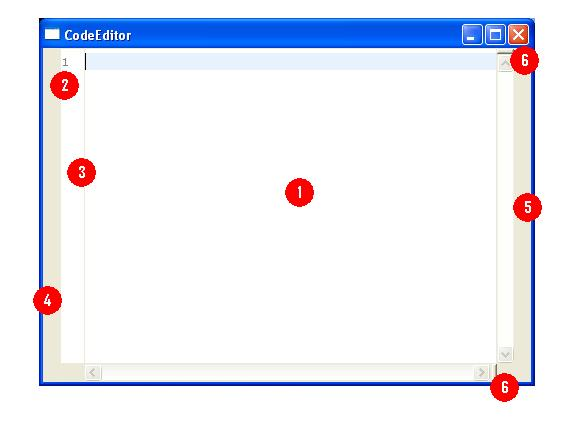
\includegraphics{images/screenshot.jpg}
\caption{EditorWidget Final Result} \label{screenshot}
\end{figure}

Figure~\ref{screenshot} shows how the end result shoud be where the numbers mean:

\begin{enumerate}
\item Editor;
\item LineNumberPanel;
\item FoldPanel;
\item LineMarksPanel;
\item OverviewLineMarksPanel;
\item Split buttons;
\end{enumerate}

\section{Editor}
As we see in section~\ref{overviewEditor} this class will extend \texttt{QTextEdit} class and add some special functionalities to it. Lets list what is spected from our Editor class:

\begin{description}
\item[Highlight current line:] Besides show a highlight rectangle on the current line, the class must provide a way to \begin{inparaenum}[\itshape a\upshape)] \item get the color of the rectangle \item set a new color to rectangle \item enable or disable this feature\end{inparaenum};

\item[Highlight current block:] If a ``Matcher'' extension is added to the editor, it should be able to paint a colored rectangle as a background to the current block of text. Analog to the \textit{highlighter} feature, editor must provide a way to \begin{inparaenum}[\itshape a\upshape)] \item get the color of the rectangle \item set a new color to rectangle \item enable or disable this feature\end{inparaenum};

\item[Goto line:] Is expected that this editor has an operation to move cursor to an especific line;

\item[Current line:] Inform the actual line number;

\item[Current column:] Inform the actual column number. This is a treak feature, as the normal \texttt{QTextEdit} class do not manage the ``\texttt{tab}'' character as a sequence of ``\texttt{space}'' characters, we have to calculate the actual column based on a \textit{tabstop} feature;

\item[Tabstop:] This is the amount of ``\texttt{space}'' characters that a ``\texttt{tab}'' character should represent. Editor must provite a way to \begin{inparaenum}[\itshape a\upshape)] \item get the tabstop value \item set a new tabstop value \item defines if editor uses the ``\texttt{tab}'' character or the ``\texttt{space}'' one to represent a tabstop\end{inparaenum};

\item[Identation:] Primary editor must repeat the white spaces used at the beggining of the previous line and if an ``Identer'' extention is defined, on each new line this extention should be called to perform an identation on the new line;

\item[Persisten selection:] Should be possible to user \begin{inparaenum}[\itshape a\upshape)] \item enters or leaves the persistent selection state \item knows if editor is in the persistent selection state\end{inparaenum};

\item[Multiline edition:] Should be possible to user \begin{inparaenum}[\itshape a\upshape)] \item enters or leaves the multiline edition state \item knows if editor is in the multiline edition state\end{inparaenum};

\end{description}

As the paintEvent will be reimplemented to fit on the stateful mode, it is need to guarantee that cursor will blink from time to time too.

Besides this features, it will be needed to reimplement some protected operations from the \texttt{QTextEdit} class:

\begin{itemize}
\item \texttt{void paintEvent(QPaintEvent *e);}
\item \texttt{void timerEvent(QTimerEvent *e);}
\item \texttt{void keyPressEvent(QKeyEvent *e);}
\item \texttt{void dragEnterEvent(QDragEnterEvent *e);}
\item \texttt{void dragLeaveEvent(QDragLeaveEvent *e);}
\item \texttt{void dragMoveEvent(QDragMoveEvent *e);}
\item \texttt{void dropEvent(QDropEvent *e);}
\item \texttt{void mousePressEvent(QMouseEvent *e);}
\item \texttt{void mouseReleaseEvent(QMouseEvent *e);}
\item \texttt{void mouseDoubleClickEvent(QMouseEvent *e);}
\item \texttt{void mouseMoveEvent(QMouseEvent *e);}
\item \texttt{QMimeData* createMimeDataFromSelection();}
\end{itemize}

From the above list, only ``\texttt{void timerEvent(QTimerEvent *e)}'' should not be a state task, other actions are stateful. Figure~\ref{editor} illustrate better this.

\begin{figure}[hbt]
\centering
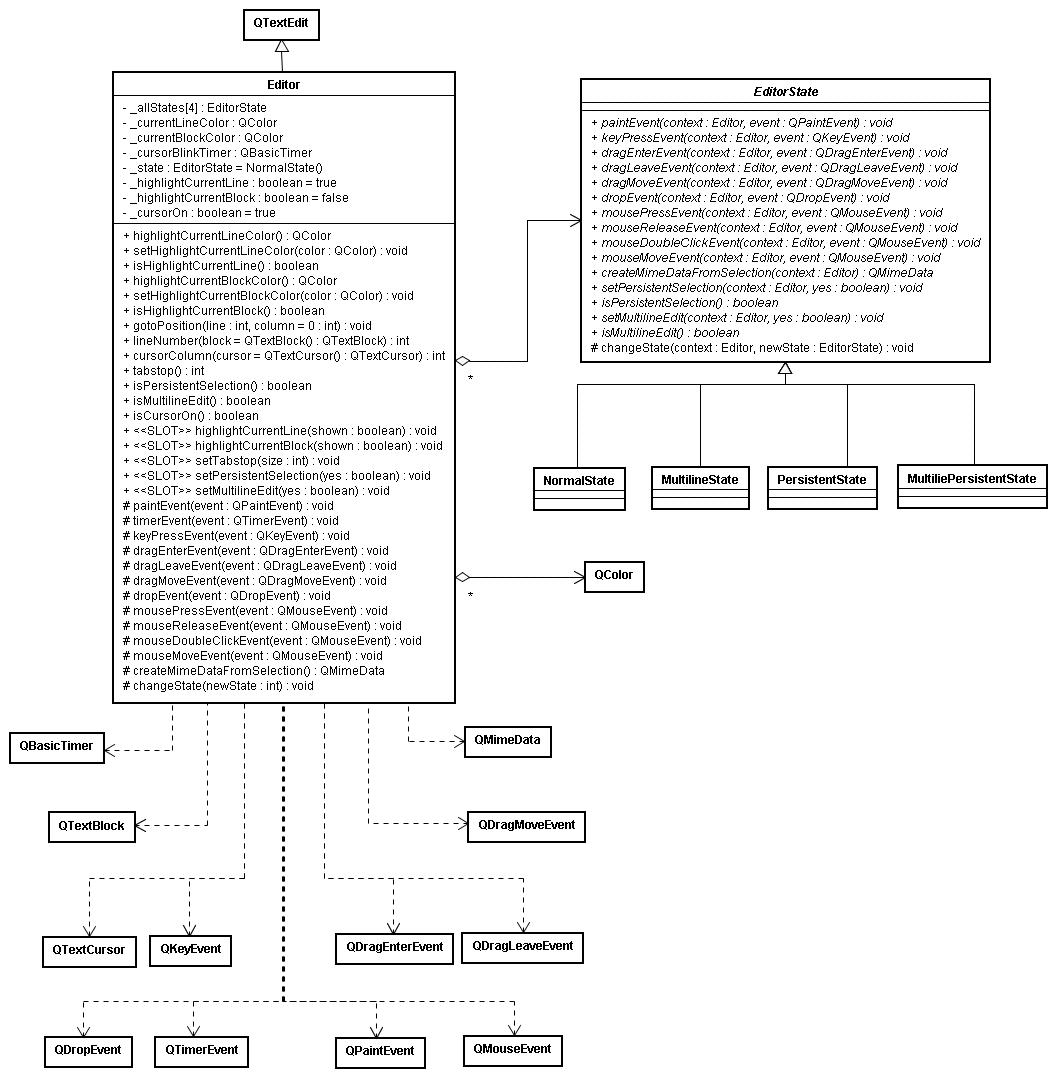
\includegraphics[width=\columnwidth]{images/editor.jpg}
\caption{Editor Diagram} \label{editor}
\end{figure}

As showed on figure~\ref{editor} besides the Editor class its necessary to implement 5 more classes to achieve the expected result:

\begin{enumerate}
\item EditorState
\item NormalState
\item MultilineState
\item PersistentState
\item MultilinePersistentState
\end{enumerate}

To have a State Pattern fully implemented, it is needed to delegate some operations to the object states, so, when implement a method that is declared on the EditorState, Editor must do the following call:

\begin{verbatim}
   _state->method(this, parameters);
\end{verbatim}

Lets see how the Editor's header will be:

\begin{verbatim}
 1. #include <QTextEdit>
 2. #include <QColor>
 3. #include <QTextBlock>
 4. #include <QTextCursor>
 5. #include <QBasicTimer>
 6.
 7. class QDragEnterEvent;
 8. class QDragLeaveEvent;
 9. class QDragMoveEvent;
10. class QDropEvent;
11. class QMouseEvent;
12. class QMimeData;
13. class EditorState;
14. 
15. class Editor : public QTextEdit {
16.     public:
17.         enum States {
18.             NormalState = 0,
19.             MultilineState = 1,
20.             PersistentState = 2,
21.             MultilinePersistentState = 3,
22.             MaxStates = 4,
23.         };
24. 
25.     public:
26.         bool   isHighlighCurrentLine();
27.         void   setHighlighCurrentLineColor(QColor color);
28.         QColor highlighCurrentLineColor();
29.         bool   isHighlighCurrentBlock();
30.         void   setHighlighCurrentBlockColor(QColor color);
31.         QColor highlighCurrentBlockColor();
32.         void   gotoPosition(int line, int column = 0);
33.         int    lineNumber(QTextBlock block = QTextBlock());
34.         int    cursorColumn(QTextCursor cursor = QTextCursor());
35.         int    tabstop();
36.         void   replaceTabWithSpaces(bool yes);
37.         bool   isPersistentSelection();
38.         bool   isMultilineEdition();
39.         bool   isCursorOn();
40.         EditorState* getState(States s) { return _allStates[s]; }
41. 
42.     public slots:
43.         void   setHighlighCurrentLine(bool shown);
44.         void   setHighlighCurrentBlock(bool shown);
45.         void   setTabstop(int size);
46.         void   setPersistentSelection(bool yes);
47.         void   setMultilineEdition(bool yes);
48. 
49.     protected:
50.         friend class EditorState;
51.
52.         void   paintEvent(QPaintEvent *e);
53.         void   timerEvent(QTimerEvent *e);
54.         void   keyPressEvent(QKeyEvent *e);
55.         void   dragEnterEvent(QDragEnterEvent *e);
56.         void   dragLeaveEvent(QDragLeaveEvent *e);
57.         void   dragMoveEvent(QDragMoveEvent *e);
58.         void   dropEvent(QDropEvent *e);
59.         void   mousePressEvent(QMouseEvent *e);
60.         void   mouseReleaseEvent(QMouseEvent *e);
61.         void   mouseDoubleClickEvent(QMouseEvent *e);
62.         void   mouseMoveEvent(QMouseEvent *e);
63.         QMimeData* createMimeDataFromSelection();
64.
65.         void changeState(EditorState*);
66. 
67.     private:
68.         EditorState* _allStates[MaxStates];
59
70.         QColor       _currentLineColor;
71.         QColor       _currentBlockColor;
72
73.         QBasicTimer  _cursorBlinkTimer;
74
75.         EditorState* _state;
76
77.         bool         _highlightCurrentLine;
78.         bool         _highlightCurrentBlock;
79.         bool         _cursorOn
80. };
\end{verbatim}

Note that I modify a little the State Pattern adding an attribute to store all possible states on the context class. I decide to do this becouse the State Pattern assumes that never will exist a copy of a state on the system. As our states are relative to editor and this editor could have a copy from himself, the states could have a copy too; for this reason a state is unique relativaly to its editor.

\subsection{EditorState}
This class is an abstract class that is the parent of all states on the editor. The only method that it provides is the \texttt{changeState} one, just to easyly the use of it from its children.

Lets see the EditorState header:

\begin{verbatim}
 1. class Editor;
 2. 
 3. class EditorState {
 4.     public:
 5.         virtual void paintEvent(Editor* context, 
                                           QPaintEvent *e) { }
 6.         virtual void keyPressEvent(Editor* context, 
                                             QKeyEvent *e) { }
 7.         virtual void dragEnterEvent(Editor* context, 
                                       QDragEnterEvent *e) { }
 8.         virtual void dragLeaveEvent(Editor* context, 
                                       QDragLeaveEvent *e) { }
 9.         virtual void dragMoveEvent(Editor* context, 
                                        QDragMoveEvent *e) { }
10.         virtual void dropEvent(Editor* context, 
                                            QDropEvent *e) { }
11.         virtual void mousePressEvent(Editor* context, 
                                           QMouseEvent *e) { }
12.         virtual void mouseReleaseEvent(Editor* context, 
                                           QMouseEvent *e) { }
13.         virtual void mouseDoubleClickEvent(Editor* context, 
                                           QMouseEvent *e) { }
14.         virtual void mouseMoveEvent(Editor* context, 
                                           QMouseEvent *e) { }
15.         virtual QMimeData* createMimeDataFromSelection(
                                          Editor* context) { }
16.         virtual bool isPersistentSelection(
                                         Editor* context) = 0;
17.         virtual void setPersistentSelection(
                               Editor* context, bool yes) = 0;
18.         virtual bool isMultilineEdit(Editor* context) = 0;
19.         virtual bool setMultilineEdit(Editor* context, 
                                                bool yes) = 0;
20. 
21.     protected:
22.         void changeState(Editor* context, 
                                       EditorState* newState);
23. };
\end{verbatim}

As a normal State Pattern implementation, the \texttt{changeState} method must be implemented like is showed in \cite{designPatterns}:

\begin{verbatim}
1. #include "editorstate.h"
2. #include "editor.h"
3. 
4. void EditorState::changeState(Editor* context, 
                                       EditorState* newState) {
5.     context->changeState(newState);
6. }
\end{verbatim}

The \texttt{friend} attribute on \texttt{Editor} class allow \texttt{EditorState} to access a protected function from it.

\subsection{NormalState}
This state do not need anything else besides what a normal \texttt{QTextEdit} class provides to realize all its functions.

The only thing that should be notted is the four pure virtual methods inherited from \texttt{EditorState} class:

\begin{verbatim}
 1. bool NormalState::isPersistentSelection(Editor* context) {
 2.     return false;
 3. }
 4.
 5. void NormalState::setPersistentSelection(Editor* context, 
                                                   bool yes) {
 6.     if (yes)
 7.         changeState(context, 
                  context->getState(Editor::PersistentState));
 8. }
 9.
10. bool NormalState::isMultilineSelection(Editor* context) {
11.     return false;
12. }
13.
14. void NormalState::setMultilineSelection(Editor* context, 
                                                   bool yes) {
15.     if (yes)
16.         changeState(context, 
                   context->getState(Editor::MultilineState));
17. }
\end{verbatim}

\subsection{MultilineState}
As describrd in \cite{functional} when editor is in this state it should be able to edit more than one line at the same time. To achieve this we need to store as mutch \texttt{QTextCursor} as necessary (actualy one per line precisely).

To select more than one line to edit user will use the selection mechanism. When he selects a text from left to right or vice versa, the selection mechanism should work as the same way that it does on the normal state, but when user selects from top to botton or vice versar, editor should add or remove lines to edit in multiline state.

So, if you have cursor at some position than you select to down (hold the \texttt{Shift} key while press the \texttt{Down Arrow} key), text cursor will grow to allow you to edit two lines at the same time. If now you select to up, editor will remove the last line from multiline edition. This behaviour is simetric and not static.

While in ``Multiline State'' somethings must be notted:

\begin{itemize}
\item Cursor never changes line automaticaly. If you are at the beginning of the line and press \texttt{Left Arrow} key, cursor will stay in that position and will not go to the end of the previous line (the samething is valid to the end of the line);

\item If user is editing more than one line and he selects a text horizontaly, all edited lines must select the text;

\item Horizontal selection never selects more than the size of the smallest edited line;

\item If more than one line is selected to edition and user moves cursor verticaly without holding the \texttt{Shift} key, all edited lines are removed and cursor must be placed on the desired position;

\item If cursor is on some position of a line and the next line do not has many characters as the actual line and user tries to grow the multiline cursor to that line, the operation is not allowed as showed in figure~\ref{multilineBlockExample}.

\begin{figure}[hbt]
\centering
\begin{tabular}{|c|ccccccc|}
\hline
 & \verb'A' & \verb'B' & \verb'C' & \verb'D' & \verb'E' & \verb'F' & \verb'G' \\ 
\hline
\verb'1' & a & a & a & a & a &   &  \\ 
\verb'2' & b & b & b & b &\vline b & b & b \\ 
\verb'3' & c & c & c &   &   &   &   \\ 
\verb'4' & d & d & d & d & d & d &   \\
\hline
\end{tabular}
\caption{Multiline State blocks selection} \label{multilineBlockExample}
\end{figure}

If cursor is on \texttt{E2} position (as showed on figure~\ref{multilineBlockExample}) and user try to ``select down'', this operation is blocked and cursor stays with the same size at the same position (note that if user selects to up the operation is allowed);

\end{itemize}

Lets see how the four pure virtual methods inherited from \texttt{EditorState} class will looks like for this state:

\begin{verbatim}
 1. bool MultilineState::isPersistentSelection(Editor* context) {
 2.     return false;
 3. }
 4.
 5. void MultilineState::setPersistentSelection(Editor* context, 
                                                   bool yes) {
 6.     if (yes)
 7.         changeState(context, 
            context->getState(Editor::MultilinePersistentState));
 8. }
 9.
10. bool MultilineState::isMultilineSelection(Editor* context) {
11.     return true;
12. }
13.
14. void MultilineState::setMultilineSelection(Editor* context, 
                                                   bool yes) {
15.     if (!yes)
16.         changeState(context, 
                   context->getState(Editor::NormalState));
17. }
\end{verbatim}

It is important to say that when changing state from ``Normal'' state to this one, the cursor selection must be converted in a multiline selection and when changing from this state to ``Normal'' one, multiline selection must be converted on a single selection.

\begin{figure}[hbt]
\centering
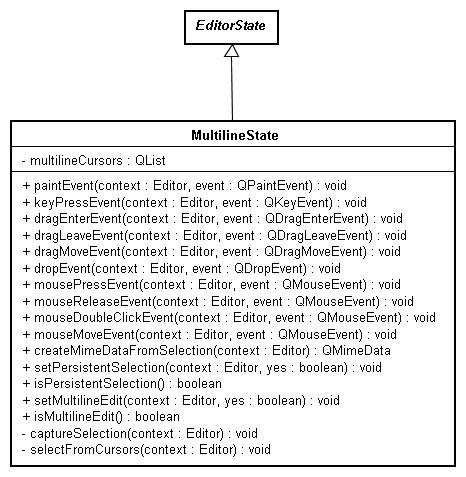
\includegraphics{images/multilinestate.jpg}
\caption{Multiline State Class Diagram} \label{multilinestate}
\end{figure}

\subsection{PersistentState}
On this state user has the flexibilty to edit a text while some other part of the text is selected without loosing selection, as said on \cite{functional}.

\begin{itemize}
\item Every state behaviour is equals to the ``Normal State'' one with exception of the selection;

\item If user inserts a text inside a selection, than selection should grow to fit the old selection plus the new text added;

\item If user inserts a text before selection, selection should walk as text is inserted;

\end{itemize}

To achieve the expected behaviour we need a \texttt{QTextCursor} to store the persistent selection on the state. So, the class diagram should looks like figure~\ref{persistentstate}.

\begin{figure}[hbt]
\centering
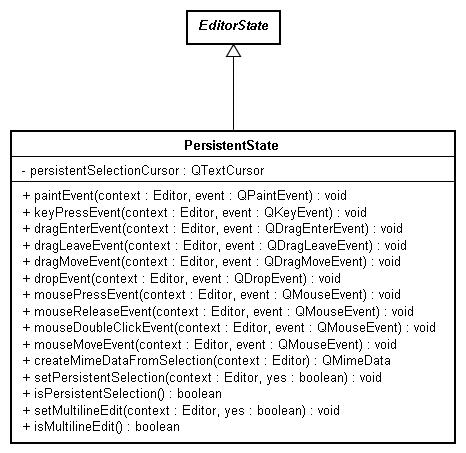
\includegraphics{images/persistentstate.jpg}
\caption{Persistent Selection State Class Diagram} \label{persistentstate}
\end{figure}

Lets see how the four pure virtual methods inherited from \texttt{EditorState} class will looks like for this state:

\begin{verbatim}
 1. bool PersistentState::isPersistentSelection(Editor* context){
 2.     return true;
 3. }
 4.
 5. void PersistentState::setPersistentSelection(Editor* context, 
                                                   bool yes) {
 6.     if (!yes)
 7.         changeState(context, 
                         context->getState(Editor::NormalState));
 8. }
 9.
10. bool PersistentState::isMultilineSelection(Editor* context) {
11.     return false;
12. }
13.
14. void PersistentState::setMultilineSelection(Editor* context, 
                                                   bool yes) {
15.     if (yes)
16.         changeState(context, 
            context->getState(Editor::MultilinePersistentState));
17. }
\end{verbatim}

\subsection{MultilinePersistentState}
This state is a sum of the two previous states, with nothing more to add figure~\ref{multilinepersistentstate} illustrates how the class diagram should looks like.

\begin{figure}[hbt]
\centering
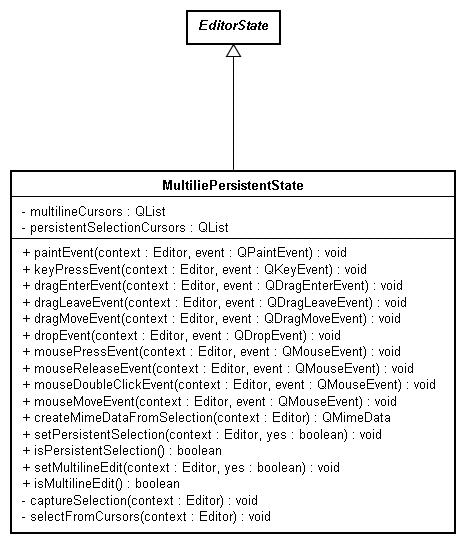
\includegraphics{images/multilinepersistentstate.jpg}
\caption{Multiline Edit with Persistent Selection State Diagram} \label{multilinepersistentstate}
\end{figure}

Lets see how the four pure virtual methods inherited from \texttt{EditorState} class will looks like for this state:

\begin{verbatim}
 1. bool MultilinePersistentState::isPersistentSelection(
                                           Editor* context){
 2.     return true;
 3. }
 4.
 5. void MultilinePersistentState::setPersistentSelection(
                                Editor* context, bool yes) {
 6.     if (!yes)
 7.         changeState(context, 
                 context->getState(Editor::MultilineState));
 8. }
 9.
10. bool MultilinePersistentState::isMultilineSelection(
                                          Editor* context) {
11.     return true;
12. }
13.
14. void MultilinePersistentState::setMultilineSelection(
                                Editor* context, bool yes) {
15.     if (!yes)
16.         changeState(context, 
                context->getState(Editor::PersistentState));
17. }
\end{verbatim}

\section{LineNumberPanel} \label{linenumbersection}
This class is a simple \textit{widget} that shows line numbers of the text edited by \texttt{Editor} class.

Althow it appears to be simple, \texttt{LineNumberPanel} is the core class of the information classes. It is responsable to store all informations of all lines in the text. The reason to use one class to store all informations is performance, if we use each class to store its own information, we will need to scan all lines of the text for each time we want a diferent information.

Allowing \texttt{LineNumberPanel} to do all the dirty work, we just need to access gethered information after it has beeing updated. 

Other important feature to be notted is the ability to expand the width of the panel as line number grows, so, the width of the \texttt{LineNumberPanel} is the size of the width of the greatest line number on the edited text.

Besides this feature, the class must provide a way to:

\begin{itemize}
\item Defines the color of the line number;
\item Get the color of the line number;
\item Set numbers font;
\item Get numbers font;
\end{itemize}

Figure~\ref{linenumberpanel} shows how this class should looks like.

\begin{figure}[hbt]
\centering
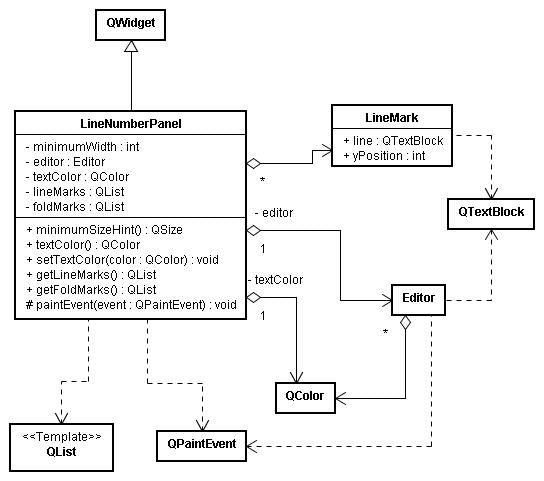
\includegraphics{images/linenumberpanel.jpg}
\caption{LineNumberPanel Class Diagram} \label{linenumberpanel}
\end{figure}

The best time to get all informations needed by all ``info panels'' is the paint event that is called every time the \texttt{Editor} class is updated. So, in this time we scan all lines of the text, store all informations needed for each line and shown \texttt{LineNumberPanel} informations, figure~\ref{linenumberpaint} shows like this precess should be.

\begin{figure}
\centering
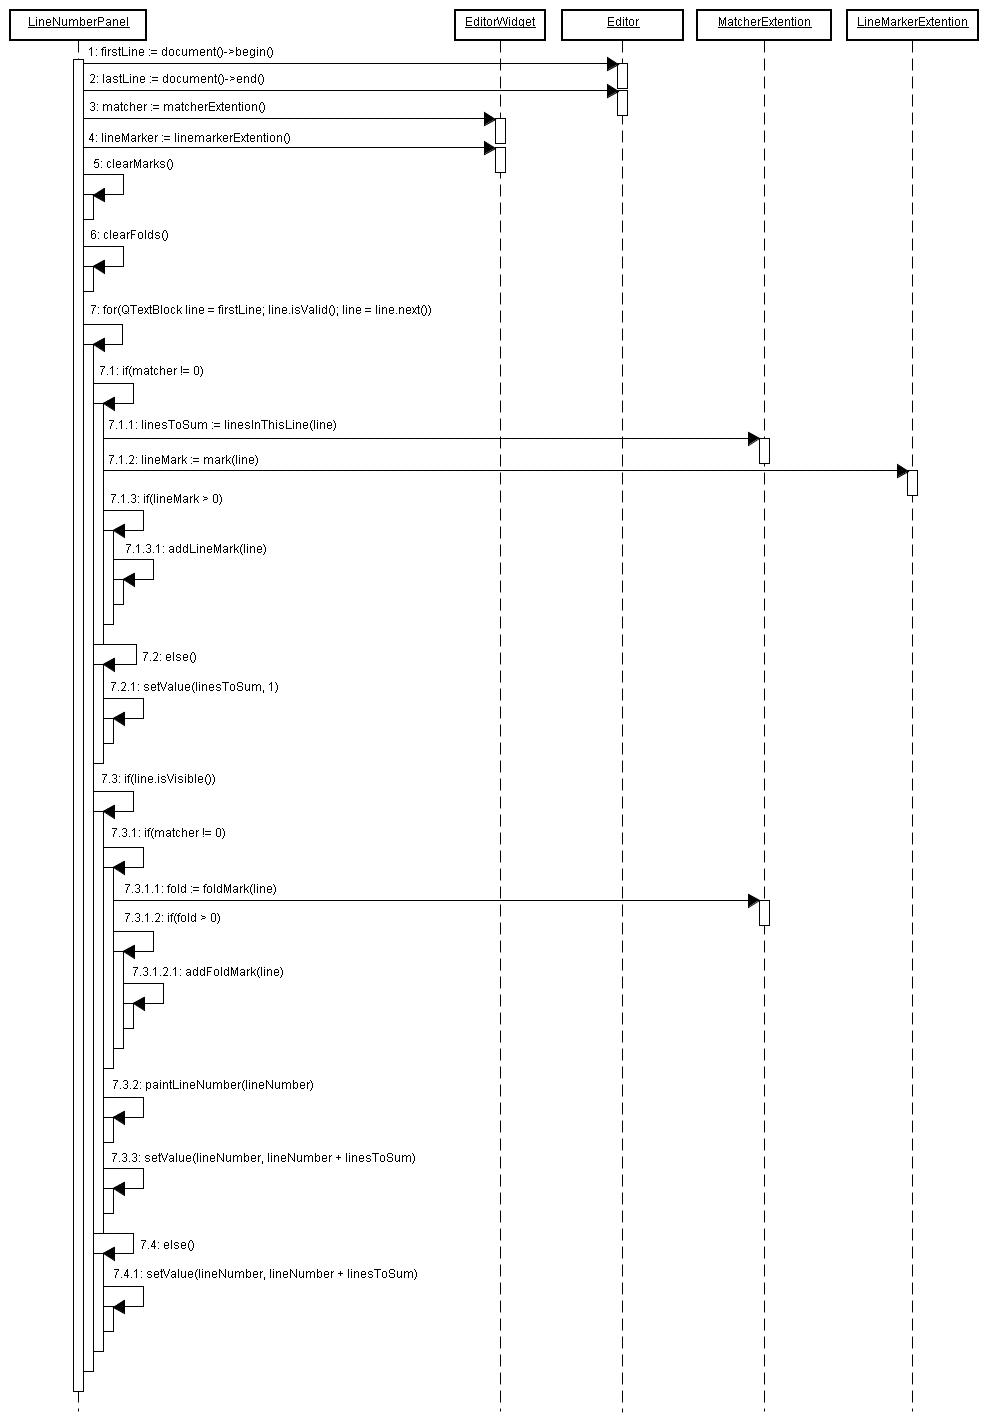
\includegraphics{images/linenumberpaint.jpg}
\caption{LineNumberPanel Paint Sequence Diagram} \label{linenumberpaint}
\end{figure}

As you can see on figure~\ref{linenumberpaint} this class interact with editor's extentions (\texttt{MatcherExtention} in this case), this extentions will be presented later in this document, but for now it is important to know that \texttt{LinemarkExtention} and \texttt{MatcherExtention}, that are used on ``info panels'', access an user data stored on each line of the text to provide informations like possibility to fold a part of the text and markers setted for an especific line.

Its also possible to note that only line marks are stored for all lines of the edited text, this is becouse the folding information is only needed for visible lines.

\section{FoldPanel}
This class is a widget that provides an icon to indicate the possibility to fold or unfold a part of the text and if user click on this icons the fold or unfold operation must be performed.

As we see on section~\ref{linenumbersection} this information is gethered by \texttt{LineNumberPanel} class, so, we need a pointer to access its informations as we need to access editor's text informations. Figure~\ref{foldpanel} shows how this class should be.

\begin{figure}[hbt]
\centering
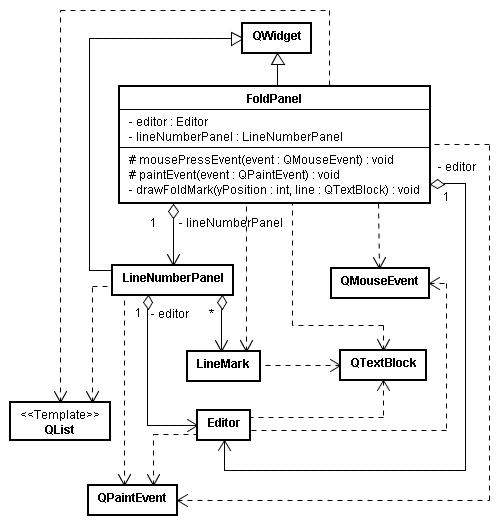
\includegraphics{images/foldpanel.jpg}
\caption{FoldPanel Class Diagram} \label{foldpanel}
\end{figure}

As we do not need to scan all lines of the text to know what line could fold or unfold, the process to show this icons is more simple than the \texttt{LineNumberPanel}'s one, figure~\ref{foldpanelpaint} illustrate this.

\begin{figure}[hbt]
\centering
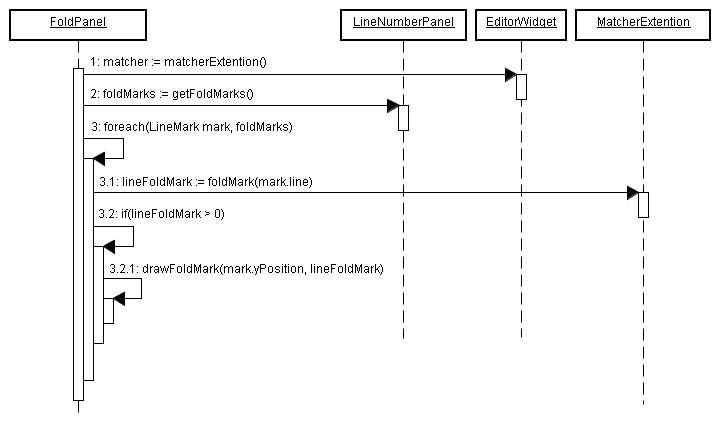
\includegraphics{images/foldpanelpaint.jpg}
\caption{FoldPanel Paint Sequence Diagram} \label{foldpanelpaint}
\end{figure}

The process to fold or unfold a line is very simple too. We just need to compare the click position with fold marks' position and if we have a match, call the \texttt{doFold} operation of the matcher extention.

\section{LineMarksPanel}
This class shows an a panel all non-fold marks of the visible lines of the text. This marks are represented by an icon that is provided by the \texttt{LinemarkerExtention} which also provides the marks itself, so, the \texttt{LinemarkerExtention} inform to \texttt{LineMarksPanel} which marks it could tread and provide an icon and a color to each mark.

The \texttt{LineMarksPanel} must treat four possible user interations:

\begin{description}
\item [Normal click above a mark:] this operation should call a defauld action to the mark;
\item [Right click above a mark:] shows a popup menu that besides other things allow user to remove the mark;
\item [Right click above an empty space:] shows a popupmenu that allow the inclusion of a new mark;
\item [Double click an empty space:] add the default mark to the desired line;
\end{description}

A text line could has mare than one mark but \texttt{LineMarksPanel} show anly the top mark. The order af a mark is given by the \texttt{LinemarkerExtention}, so, this class should never worrie about it.

Other thing to say is about popup menus. The panel must ask to \texttt{LinemarkerExtention} to marks popup menu, this way its possible to have on the popup menu all marks of the line on the fly.

Figure~\ref{linemarkspanel} illustrate how this class should looks like.

\begin{figure}[hbt]
\centering
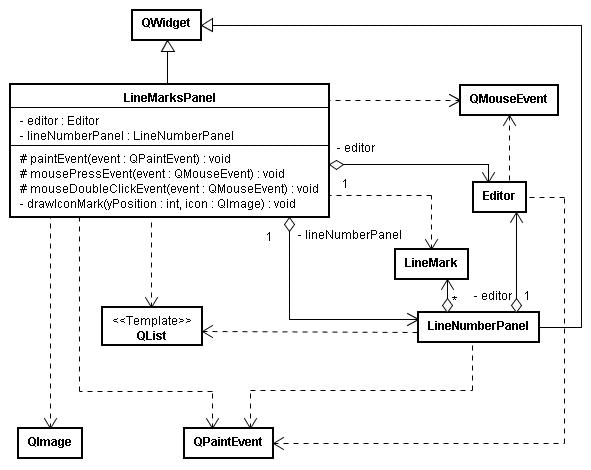
\includegraphics{images/linemarkspanel.jpg}
\caption{LineMarksPanel Class Diagram} \label{linemarkspanel}
\end{figure}

As ocour with \texttt{FoldPanel} the paint event is quite simple, the only thing to worry about is that \texttt{LineNumberPanel} get marks from \textbf{all} lines, so, its important to filter this and show only the visible ones. The figure~\ref{linemarkspanelpaint} should illustrate better this.

\begin{figure}[hbt]
\centering
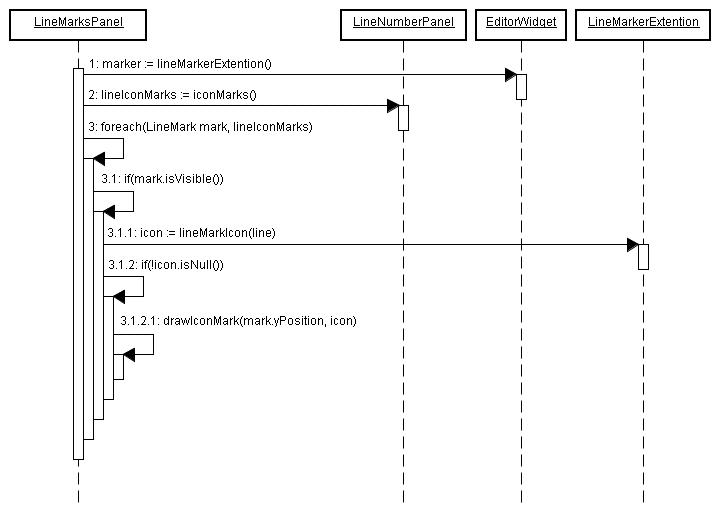
\includegraphics{images/linemarkspanelpaint.jpg}
\caption{LineMarksPanel Paint Sequence Diagram} \label{linemarkspanelpaint}
\end{figure}

The interaction methods are simple too, its needed to scan all visible marks and compare the click position to each mark position and if a mark is clicked than call the right method of \texttt{LinemarkerExtention} to treat each event.

\section{OverviewLineMarksPanel}
As the name says, this class should show all marks of the text at the same time. This is achieved by representing the text as the entire panel area and line marks as little rectangles that are positioned on the panel relatively to the line on the text.

If user clicks on a mark rect, editor must position text cursor on the line of the mark. Figure~\ref{overviewmarkspanel} shows how this class should looks like.

\begin{figure}[hbt]
\centering
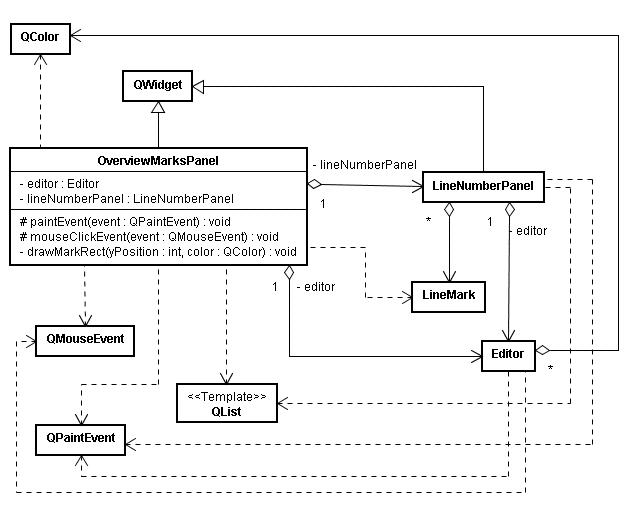
\includegraphics{images/overviewmarkspanel.jpg}
\caption{OverviewLineMarksPanel Class Diagram} \label{overviewmarkspanel}
\end{figure}

The paint event of this panel is even easyer than \texttt{LineMarksPanel} ones. It not needs to check if a mark is visible or not as it will show ``all'' marks of the text. Lets see on figure~\ref{overviewmarkspanelpaint} how this sequence should looks like.

\begin{figure}[hbt]
\centering
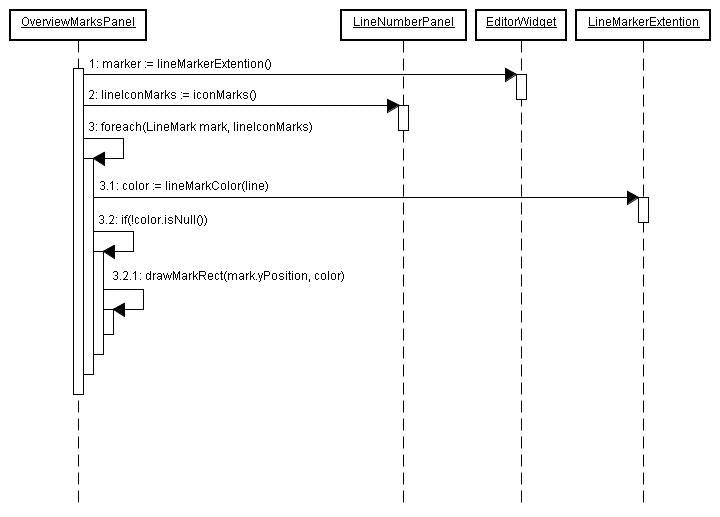
\includegraphics{images/overviewmarkspanelpaint.jpg}
\caption{OverviewLineMarksPanel Paint Sequence Diagram} \label{overviewmarkspanelpaint}
\end{figure}

When user clicks on a mark, \texttt{OverviewLineMarksPanel} must call editor's method to go to a new line to position its cursor on the desired mark.

\bibliography{technical}
\bibliographystyle{ieeetr}

\end{document}
